
\section{Existing Frameworks: Double-DOP and DOP$^*$}
%A description and comparison of Double-DOP and DOP*

A PTSG consists of the symbolic grammmar, i.e. a set of fragments, and the corresponding weights. In the general case of DOP, all fragments are extracted from all the trees in the treebank. The number of fragments is exponential in the length of the sentences, thus the total number of fragments extracted would be far too large for efficient computation. 
%DOP1: sample
Later models have therefore restricted the set of fragments in the grammar, thus improving computational efficiency. However, determining a proper subset of fragments to use is not trivial and this choice may negatively influence the performance of the grammar.

%Iets met Goodman? Die behoudt alleen kleine stukjes en speciale regels, maar daardoor geen expliciete representatie van 'productive units' (Sangati, einde van sectie 2)

In this section, we outline two approaches to constrain the extraction of fragments: \ddop and \dops. Furthermore, we discuss the similarities and dissimilarities for these two approaches. 

\subsection{\ddop}
In the following, we discuss \ddop{} as it was presented in \cite{sangati2011}. In this model, no unique fragments are extracted from the dataset: if a construction occurs in one tree only, it is probably not representative for the language. This is carried out by a dynamic algorithm using tree-kernels. It iterates over pairs of trees in the treebank, looking for fragments they have in common. In addition, only the largest shared fragment is stored. 

The symbolic grammar that is the output of this algorithmis not guaranteed to derive each tree in the training corpus. Therefore all one-level fragments, consitutuing the set of PCFG-productions, are also added.

After the extraction of the symbolic grammar, the weights are obtained. This is done in a second pass over the treebank, assessing the relative frequencies. 

The \ddop{} model has its main focus on determining the symbolic grammar. However, it was implemented with different estimators and maximizing objectives. Empirical results show that %

\paragraph{Consistency and bias}

\subsection{\dops}
In \dops{} \cite{zollmann2005}, a rather different approach is taken called held-out estimation. The treebank is split in two parts, the extraction corpus ($EC$) and a held-out corpus ($HC$). An initial set of fragments is extracted from the $EC$, containing all the fragments from its trees. The weights are then determined so as to to maximize the likelihood of $HC$, under the assumption that this is equivalent to maximizing the joint probability of the \emph{shortest derivations} of the trees in $HC$. All fragments that do not occur in such a derivation are removed from the symbolic grammar. Note that some trees in $HC$ may not be derivable at all. 

\paragraph{Consistency and bias}
\dops{} was claimed to be the first consistent (non-trivial) DOP-estimator, \cite{zollmann2005} provides a consistency proof. On the other hand \dops{} is  biased, but Zollmann shows how bias actually arises from generalization: no non-overfitting DOP estimator could be unbiased. Bias is therefore not prohibited but on the contrary a desirable property of an estimator.

In \cite{zuidema2006} it is argued that there is a problem with the consistency proof given for \dops{}, as well as the non-consistency proof for other DOP-estimators by \cite{johnson2002}. Zuidema points out that these proofs use a frequency-distribution test, whereas for DOP a weight-distribution test would be more appropriate. 
%Wat hiermee?

%
%\subsection{Comparison}
%Both \dops{} and \ddop{} restrict the symbolic grammar based on some notion of reoccurence of fragments. 
%
%In \ddop{} this is evident, it is explicit in the algorithm how (largest) reoccuring fragments are added to the grammar. From a computational point of view, this approach is very intuitive and can be implemented rather efficiently. However, the threshold (two) on the number of reoccurences might seem rather trivial. Indeed, \cite{sangati2011} reports experiments varying this threshold that show how performance drops for higher thresholds, with on the other hand a great reduction of the size of the grammar. A proper setting might well depend on the size and nature of the treebank used, and the computational costs one is willing to pay. In short, \ddop{} is computationally attractive but its theoretical foundation is not convincing us.
%%wel performance maar competence raadsel
%
%Theoretically,\dops{} is more appealing: we decide on the symbolic grammar by assessing which fragments are actually used in derivations. The main assumption is that shortest derivations are preferred. The splitting of the treebank makes this possible (otherwise the grammar would be terribly overfitted).
%
%
%
%\subsection{Preview}
%\dops{} is proven to be consistent and theoretically appealing. The computational problem of \dops{} is that, at first, the entire set of possible fragments is extracted from $EC$ and this set is reduced in a later phase. This comes with the need for huge storage and computation. In the next section, we investigate the possibility of reformulating the \dops{} approach with insights from the \ddop{} model to maintain the best of both worlds. 
%
%%\dops{} theoretically more appealing, \ddop{} computationally: lend properties of \ddop{} to implement \dops{}






\subsection{Comparison}
%The theoretical properties of \dops{} and \ddop{} differ:  
\dops{} and \ddop{} differ both in the set of fragments they extract and their estimation of the weights. To investigate the exact differences, we will view both steps separately.

Note that the \dops{} extraction needs another decision: in many cases, there are several shortest derivations possible. From now on, we add all fragments that occur in one of these shortest derivations to the symbolic grammar. Of course we need to adjust the weights (e.g. divide the frequency counts by the number of shortest derivations) so that no full tree gets a higher impact on the PTSG. We will keep to the original formulation of \dops{} in case no derivation is possible, i.e. not including any fragments for this tree.

\paragraph{Extraction}
\ddop{} uses tree kernels to find the maximal overlapping fragments of pairs of trees, which are added to the symbolic grammar. We will call this the \emph{maximal-overlap} method. \dops{} iteratively finds the shortest derivation of one tree given all the fragments of a set of trees, herafter the \emph{shortest-derivation} method. The example in figure \ref{f:differentSets} shows that the sets of extracted fragments from these methods does indeed differ.

\begin{figure}
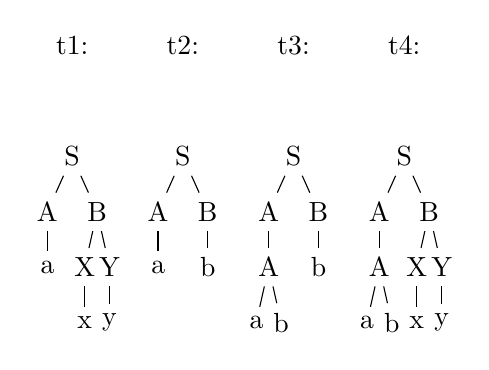
\begin{tikzpicture}
[node distance = 40 pt, sibling distance=18pt, level distance=20pt,level 2/.style={sibling distance=9pt},level 3/.style={sibling distance=9pt}]

\node (t1) {t1:}
node [ below of= t1] {S}
child {node {A} 	child {node {a}}
	}
child {node {B}	child{node {X}	child{node {x}}}
			child{node {Y}	child{node {y}}}
	}
;

\node [right of = t1] (t2) {t2:}
node [ below of= t2] {S}
child {node {A} 	child {node {a}}
	}
child {node {B}	child{node {b}}
	}
;

\node [right of = t2] (t3) {t3:}
node [ below of= t3] {S}
child {node {A} 	child {node {A}	child{node {a}}
						child{node {b}}
				}
	}
child {node {B}	child{node {b}}
	}
; 

\node [right of = t3] (t4) {t4:}
node [ below of= t4] {S}
child {node {A} 	child {node {A}	child{node {a}}
						child{node {b}}
				}
	}
child {node {B}	child{node {X}	child{node {x}}}
			child{node {Y}	child{node {y}}}
	}
;
\end{tikzpicture}
\caption{The fragment sets resulting from \emph{maximal-overlap} and \emph{shortest-derivation} extraction}
\label{f:differentSets}
\end{figure}

It is easy to see that the \dops{} extraction method does not depend on the corpus split: we can also try to find the shortest possble derivation using fragments from all the other trees. Likewise \ddop{} could be implemented using a split, comparing pairs that consist of a tree from each part of the corpus. Whether the corpus is split in two does only influence the size of the symbolic grammar and not its constitution.

Therefore, we will implement both extraction methods in a 1 vs the rest manner. In this way, we can analyse how the resulting symbolic grammars differ. The analysis will comprise the size of the resulting symbolic grammar and the relative number of fragments of certain depth. Furthermore, we might be able to find interesting patterns by manually looking at the fragments that were extracted by one of the systems only.s

\paragraph{Estimation}
The next step would be to compare the estimation methods: use either a split or the whole set of trees for both estimators. \ddop{} counts the occurences of fragments in the symbolic grammar, whereas \dops{} counts the occurrences in shortest derivations. Therefore, the extraction and estimation are best done simultaneously in the latter case. This comparison would involve a performance measure, such as the F1-score for correctly predicted parses.




























